%! Author = Len Washington III
%! Date = 4/15/2024

% Preamble
\documentclass[title={Chapter 15}]{fdsn201notes}

% Packages

% Document
\begin{document}%
%
%<*Chapter15>
\maketitle{15}{Nutrition Through the Life Cycle: Childhood to Late Adulthood}%
%Chapter 15: Nutrition Through the Life Cycle:Childhood to Late Adulthood,and In Depth 15.5, Searching For the Fountain of Youth

\section{Toddlers}\label{sec:toddlers}
\begin{itemize}
	\item Age 1 to 3 years
	\begin{itemize}
		\item Rapid growth rate of infancy begins to slow
		\item Gain 5.5 to 7.5 inches and 9 to 11 pounds
		\item High energy requirement due to increased activity level
	\end{itemize}
	\item Macronutrients
	\begin{itemize}
		\item 30--40\% of total kcal from fat
		\item 1.10 g of protein per kg body weight per day
		\item 130 g carbohydrates per day
		\item 14 g fiber per 1,000 kcal of energy consumed
	\end{itemize}
	\item Micronutrients
	\begin{itemize}
		\item Ensure adequate intake of the micronutrients obtained from fruits and vegetables, including
		\item Vitamins A, C, E; calcium; iron; zinc
		\item Calcium is necessary to promote optimal bone mass
		\item Iron-deficiency anemia is the most common nutrient deficiency in young children
	\end{itemize}
	\item Fluid needs
	\begin{itemize}
		\item 1.3 liters/day
	\end{itemize}
	\item Supplements
	\begin{itemize}
		\item Toddlers may need supplements due to their erratic eating habits, especially for fluoride
		\item Supplements should not exceed 100\% of the Daily Value for any nutrient
	\end{itemize}
\end{itemize}

\begin{table}[H]
	\centering
	\caption{Nutrients for Children and Adolescents}
	\label{tab:nutrients-for-children-and-adolescents}
	\rowcolors{2}{rowmedgreen}{rowlightgreen}
	\begin{adjustbox}{max width=0.975\paperwidth,center}
		\begin{tabular}{p{0.13\paperwidth} *{4}{p{0.22\paperwidth} }}
			\rowcolor{rowdarkgreen}%
			\textbf{Nutrient} & \textbf{Toddles (1--3) Years} & \textbf{Children (4--8) Years} & \textbf{Children (9--13) Years} & \textbf{Adolescents (14--18 Years)}\\
			\textbf{Fat} & No RDA & No RDA & No RDA & No RDA\\
			\textbf{Protein} & 1.10 g/kg body weight per day & 0.95 g/kg body weight per day & 0.95 g/kg body weight per day & 0.85 g/kg body weight per day\\
			\textbf{Carbohydrate} & 130 g/day & 130 g/day & 130 g/day & 130 g/day\\
			\textbf{Vitamin A} & 300 $\mu$g/day & 400 $\mu$g/day & 600 $\mu$g/day & Boys: 900 $\mu$g/day

			Girls: 700 $\mu$g/day\\
			\textbf{Vitamin C} & 15 mg/day & 25 mg/day & 45 mg/day & Boys: 75 mg/day

			Girls: 65 $\mu$g/day\\
			\textbf{Vitamin E} & 6 mg/day & 7 mg/day & 11 mg/day & 15 mg/day\\
			\textbf{Calcium} & 700 mg/day & 1,000 mg/day & 1,300 mg/day & 1,300 mg/day\\
			\textbf{Iron} & 7 mg/day & 10 mg/day & 8 mg/day & Boys: 11 mg/day

			Girls: 15 mg/day\\
			\textbf{Zinc} & 3 mg/day & 5 mg/day & 8 mg/day & Boys: 11 mg/day

			Girls: 9 mg/day\\
			\textbf{Fluid} & 1.3 liters/day & 1.7 liters/day & Boys: 2.4 liters/day

			Girls: 2.1 liters/day & Boys: 3.3 liters/day

			Girls: 2.3 liters/day\\
			\rowcolor{rowdarkgreen} & & & &\\
		\end{tabular}
	\end{adjustbox}
\end{table}

\begin{itemize}
	\item Nutritious food choices
	\begin{itemize}
		\item Most toddlers have an innate ability to match their intake with their needs
		\item Keeping a nutritious variety of foods available encourages a healthful diet
		\item Food should not be forced on a child
		\item Do not use bribery to encourage children to eat
		\item Foods prepared should be fun
	\end{itemize}
\end{itemize}

\begin{figure}[H]
	\centering
	
\includegraphics[width=\textwidth]{15_fun_food}
	\caption{Fun Food}
	\label{fig:fun-food}
\end{figure}

\begin{figure}[H]
	\centering
	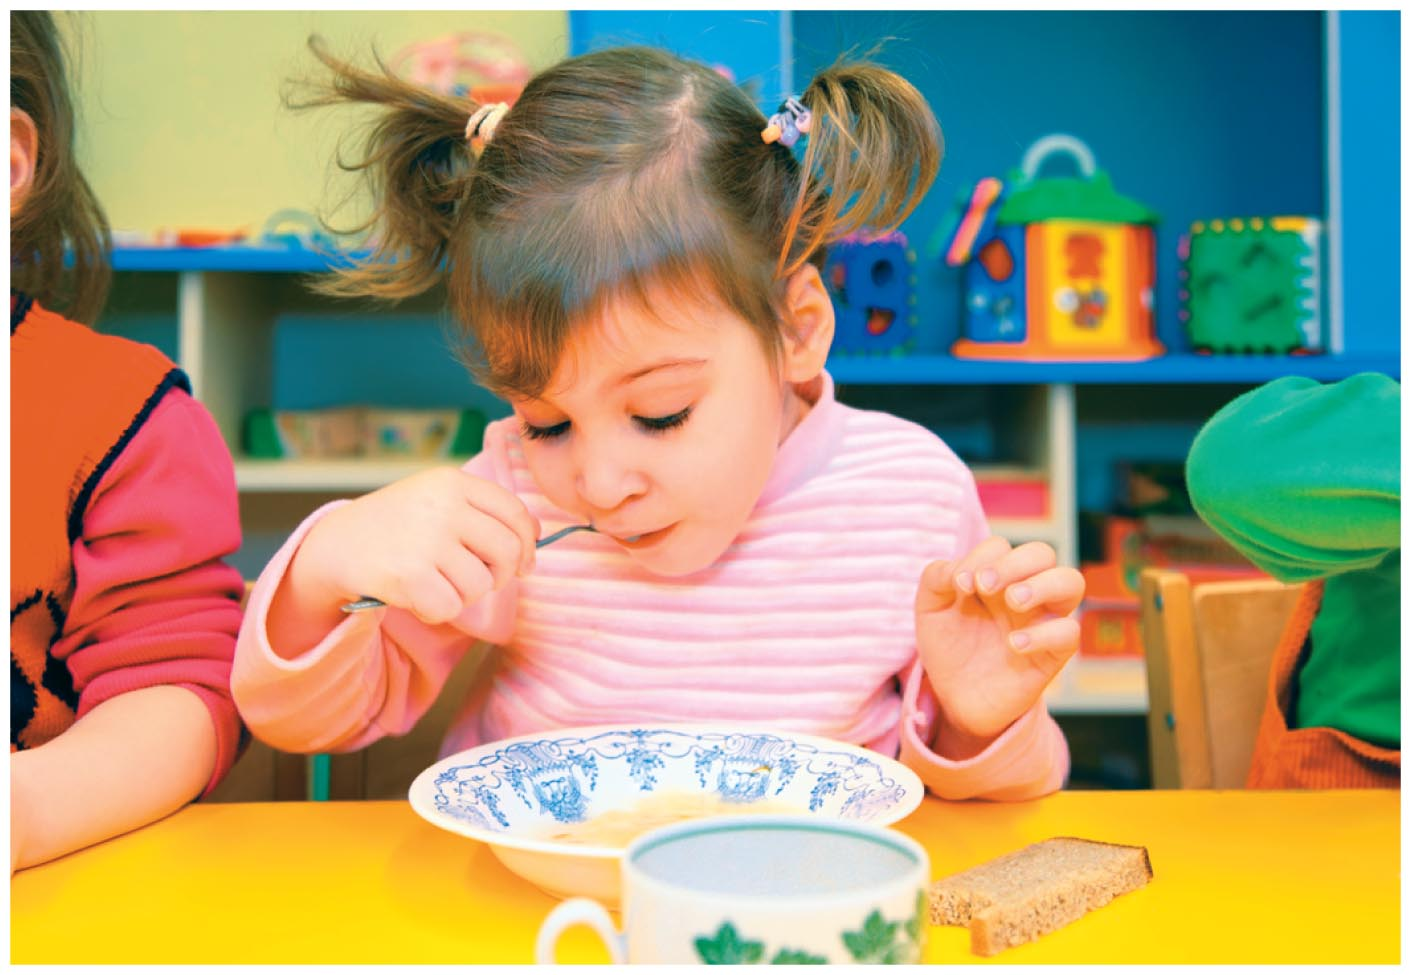
\includegraphics[width=\textwidth]{15_portion_sizes_for_preschoolers}
	\caption{Portion Sizes for Preschoolers}
	\label{fig:portion-sizes-for-preschoolers}
\end{figure}

\section{Vegan Diets for Toddlers}\label{sec:vegan-diets-for-toddlers}
\begin{itemize}
	\item Vegan diets may not be healthful for toddlers. Due  to the restriction of no foods from animal origin there are potential risks:
	\begin{itemize}
		\item Protein
		\item Calcium
		\item Zinc and iron
		\item Vitamins D and $\mbox{B}_{12}$
		\item Fiber
	\end{itemize}
\end{itemize}

\section{Young Children}\label{sec:young-children}
\begin{itemize}
	\item Age 4 to 8 years
	\begin{itemize}
		\item Dietary Reference Intake (DRI) values are the same for both boys and girls through the age of about 8
		\item Growth rate is 2 to 4 inches per year
	\end{itemize}
	\item Macronutrients
	\begin{itemize}
		\item Total fat intake should gradually drop to a level closer to adult fat intake
		\item 25--35\% of total energy from fat
		\item 0.95 g of protein per kg body weight per day
		\item 130 g carbohydrate per day
		\item 14 g fiber per 1,000 kcal of energy consumed
	\end{itemize}
	\item Micronutrients
	\begin{itemize}
		\item Vitamins and minerals from fruits and vegetables continue to be a concern
		\item Vitamins A, C, E; calcium; iron; zinc
		\item Increases in DRIs compared to toddlers
	\end{itemize}
	\item Fluid
	\begin{itemize}
		\item 1.7 liters/day (about 5–8 cups), including water
	\end{itemize}
	\item Supplements
	\begin{itemize}
		\item May be recommended when particular food groups are not eaten regularly
		\item Supplements should be appropriate for the child’s age
	\end{itemize}
\end{itemize}

\begin{figure}[H]
	\centering
	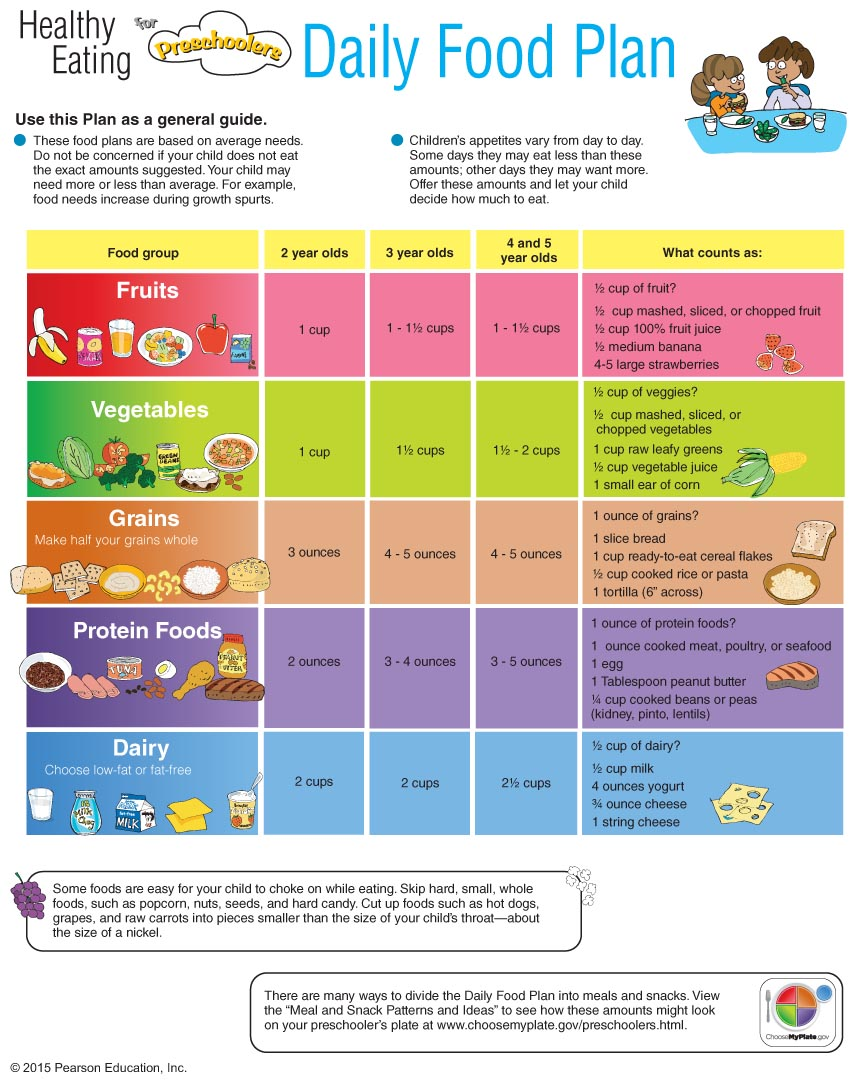
\includegraphics[width=\textwidth]{15_myplate_daily_food_plan_for_preschoolers}
	\caption{MyPlate Daily Food Plan for Preschoolers}
	\label{fig:myplate-daily-food-plan-for-preschoolers}
\end{figure}

\begin{itemize}
	\item Nutritious food choices
	\begin{itemize}
		\item Parents can teach children about healthful food choices
		\begin{itemize}
			\item Some foods “help us grow healthy and strong”
			\item Some foods are better used as occasional treats
		\end{itemize}
		\item Eating a balanced breakfast has many benefits
		\item Some school lunch programs are in need of updated and more healthful menu selections
	\end{itemize}
\end{itemize}

\section{Children: Nutrition-Related Concerns}\label{sec:children:-nutrition-related-concerns}
\begin{itemize}
	\item Overweight and obesity
	\item Dental caries
	\item Inadequate calcium intake
	\item Body image concerns
	\item Childhood food insecurity
\end{itemize}

\section{Older Children}\label{sec:older-children}
\begin{itemize}
	\item Age 9 to 13 years
	\begin{itemize}
		\item Growth is slow and steady--2 to 4 inches per year
		\item Growth is primarily driven by hormones during puberty
		\item Children begin to make their own food choices
		\item Activity levels vary
	\end{itemize}
	\item Macronutrients
	\begin{itemize}
		\item 25--35\% of total energy from fat
		\item 0.95 g protein per kg body weight per day
		\item 130 g carbohydrates per day
		\item 45--60\% of kcal from carbohydrates
		\item 14 g fiber per 1,000 kcal of energy consumed
	\end{itemize}
	\item Micronutrients
	\begin{itemize}
		\item Micronutrient needs rise sharply as children approach puberty
		\item Meeting the needs for calcium and iron is very important
	\end{itemize}
	\item Fluid
	\begin{itemize}
		\item Adequate intake (AI) of fluids varies by gender, ranging from 2.1 liters/day (females) to 2.4 liters/day (males)
	\end{itemize}
	\item Supplements
	\begin{itemize}
		\item A vitamin/mineral supplement supplying no more than 100\% of the daily values may be warranted
	\end{itemize}
	\item Nutritious food choices
	\begin{itemize}
		\item Peer pressure can influence a child’s food choices
		\item Healthy role models, such as athletes, can be used to encourage good choices
		\item School lunches must meet U.S\@.\ Department of Agriculture (USDA) guidelines, but this does not control what the child actually eats
	\end{itemize}
\end{itemize}

\section{Adolescents}\label{sec:adolescents}
\begin{itemize}
	\item Age 14 to 18 years
	\begin{itemize}
		\item Growth spurts begin at age 9 to 10 for girls and 10 to 11 for boys
		\item Weight and body composition also change
	\end{itemize}
\end{itemize}

\begin{figure}[H]
	\centering
	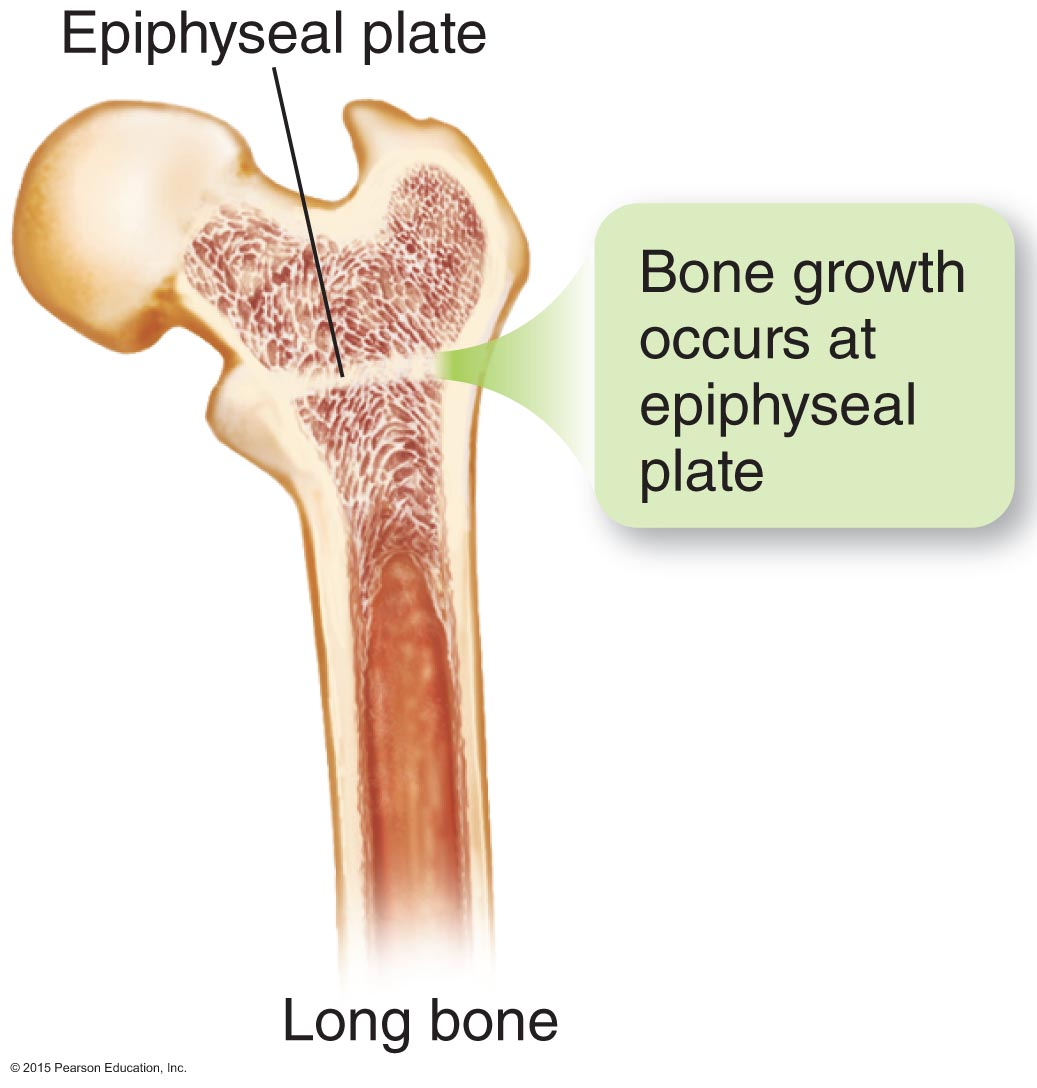
\includegraphics[width=\textwidth]{15_skeletal_growth}
	\caption{Skeletal Growth}
	\label{fig:skeletal-growth}
\end{figure}

\begin{itemize}
	\item Macronutrients
	\begin{itemize}
		\item Estimated energy requirements (EERs) for adolescents are based on gender, age, activity level, height, and weight
		\item 25–35\% of total energy from fat
		\item 45–65\% of kcal from carbohydrates
		\item 0.85 g protein per kg body weight per day
		\item 26 g of fiber per day
	\end{itemize}
	\item Micronutrients
	\begin{itemize}
		\item Calcium and vitamin D intakes must be sufficient for achieving peak bone density
		\item Iron needs are relatively high
		\begin{itemize}
			\item 15 mg/day for girls
			\item 11 mg/day for boys
		\end{itemize}
		\item Vitamin A is critical for supporting rapid growth and development
	\end{itemize}
	\item Fluid
	\begin{itemize}
		\item The need to maintain fluid intake is increased by higher activity levels
		\item Boys: 3.3 liters/day
		\item Girls: 2.3 liters/day
	\end{itemize}
	\item Supplements
	\begin{itemize}
		\item A multivitamin can be a safety net but should not replace a healthful diet
	\end{itemize}
	\item Nutritious food choices
	\begin{itemize}
		\item Peer influences and fast-paced lifestyle can lead adolescents to choose fast foods
		\item Parents can act as role models and keep healthful food choices available
		\item Adequate intake of fruits, vegetables, and whole grains should be encouraged
	\end{itemize}
	\item Nutrition-related concerns
	\begin{itemize}
		\item Bone density concerns arise from inadequate calcium intake
		\item Eating disorders and poor body image problems can begin during these years
		\item Hormonal changes are largely responsible for acne flare-ups
		\item Cigarette smoking, alcohol consumption, and illegal drug use all have a significant impact on growth and health
	\end{itemize}
\end{itemize}

\section{Pediatric Obesity}\label{sec:pediatric-obesity}
\begin{itemize}
	\item Obesity in children
	\begin{itemize}
		\item \definition{Obese}{a BMI at or above the 95th percentile}
		\item Increased risk of developing type 2 diabetes, hypertension, and other serious medical problems
	\end{itemize}
	\item Overweight children are at much greater risk of becoming overweight adults
	\item Obesity is now epidemic in the United States among school-aged children
	\item Caused by too many Calories and not enough physical activity
	\item Dietary Guidelines for Americans recommend that children be very active for at least 1 hour per day
\end{itemize}

\subsection{Prevention}\label{subsec:prevention}
\begin{itemize}
	\item Constructive support for physical activity
	\item Healthful, balanced, regular meals
	\item Developing healthful eating habits early in life
	\item Family-wide support for nutritious food choices
	\item Parental control of food purchase and preparation
	\item Minimize the amount of meals eaten out of the home, especially fast food
	\item School support for healthful food choices
	\item Daily activity and exercise
\end{itemize}

\begin{table}[H]
	\centering
	\begin{adjustbox}{max width=0.975\paperwidth,max height=0.75\paperheight,center}
		\begin{threeparttable}
			\caption{Examples of Physical Activities for Children and Adolescents}
			\label{tab:physical-activities-for-children-and-adolescents}
			\rowcolors{2}{rowmedgreen}{rowlightgreen}
			\begin{tabular}{p{0.2\paperwidth} p{0.4\paperwidth} p{0.4\paperwidth}}
				\rowcolor{rowdarkgreen}%
				\textbf{Type of Physical Activity} & \textbf{Age Group: Children} & \textbf{Age Group: Adolescents}\\
				Moderate-intensity aerobic &
				\begin{itemize}[label=\activitymark,leftmargin=0pt]
					\item Active recreation, such as hiking, skateboarding, rollerboarding
					\item Bicycle riding
					\item Brisk walking
				\end{itemize} &
				\begin{itemize}[label=\activitymark,leftmargin=0pt]
					\item Active recreation, such as canoeing, hiking, skateboarding, rollerboarding
					\item Brisk walking
					\item Bicycle riding (stationary or road bike)
					\item Housework and yard word, such as sweeping or pushing a lawn mower
					\item Games that require catching and throwing, such as baseball and softball
				\end{itemize}\\
				Vigorous-intensity aerobic &
				\begin{itemize}[label=\activitymark,leftmargin=0pt]
					\item Active games involving running and chasing, such as tag
					\item Bicycle riding
					\item Jumping rope
					\item Martial arts, such as karate
					\item Running
					\item Sports such as soccer, ice or field hockey, basketball, swimming, tennis
					\item Cross-country skiing
				\end{itemize} &
				\begin{itemize}[label=\activitymark,leftmargin=0pt]
					\item Active games involving running and chasing, such as flag football
					\item Bicycle riding
					\item Jumping rope
					\item Martial arts, such as karate
					\item Running
					\item Sports such as soccer, ice or field hockey, basketball, swimming, tennis
					\item Vigorous dancing
					\item Cross-country skiing
				\end{itemize}\\
				Muscle-strengthening &
				\begin{itemize}[label=\activitymark,leftmargin=0pt]
					\item Games such as tug-of-war
					\item Modified push-ups (with knees on the floor)
					\item Resistance exercises using body weight or resistance bands
					\item Rope or tree climbing
					\item Sit-ups (curl-ups or crunches)
					\item Swinging on playground equipment/bars
				\end{itemize} &
				\begin{itemize}[label=\activitymark,leftmargin=0pt]
					\item Games such as tug-of-war
					\item Push-ups and pull-ups
					\item Resistance exercises with exercise bands, weight machines, hand-held weights
					\item Climbing wall
					\item Sit-ups (curl-ups or crunches)
				\end{itemize}\\
				Bone-strengthening &
				\begin{itemize}[label=\activitymark,leftmargin=0pt]
					\item Games such as hopscotch
					\item Hopping, skipping, jumping
					\item Jumping rope
					\item Running
					\item Sports such as gymnastics, basketball, volleyball, tennis
				\end{itemize} &
				\begin{itemize}[label=\activitymark,leftmargin=0pt]
					\item Hopping, skipping, jumping
					\item Jumping rope
					\item Running
					\item Sports such as gymnastics, basketball, volleyball, tennis
				\end{itemize}\\
				\rowcolor{rowdarkgreen} & & \\
			\end{tabular}
			\begin{tablenotes}
				\small
				\item \textit{*Note:} Some activities, such as bicycling, can be moderate or vigorous intensity, depending on level of effort.

				\textit{Source:} Data from \textit{2008 Physical Activity Guidelines for Americans,} U.S\@.\ Department of Health and Human Services.
			\end{tablenotes}
		\end{threeparttable}
	\end{adjustbox}
\end{table}

\section{Older Adults}\label{sec:older-adults}
\begin{itemize}
	\item Physiologic changes to the bodies of older adults, age 65 years and older, include
	\begin{itemize}
		\item Decreased muscle and lean tissue
		\item Increased fat mass
		\item Decreased bone density
		\item Impaired absorption of nutrients
		\item Taste and smell perception is often diminished
	\end{itemize}
	\item Macronutrients
	\begin{itemize}
		\item Energy needs usually decrease due to reduced activity levels and lower lean body mass
		\item General recommendations for fat, carbohydrate, and protein intakes are the same as for younger adults
		\item Recommended to not consume more than 30\% of energy from sugars
		\item Fiber recommendations are slightly lower for older adults
	\end{itemize}
	\item Micronutrients
	\begin{itemize}
		\item Calcium and vitamin D requirements increase due to poor calcium absorption
		\item Iron needs decrease
		\item Zinc intake should be maintained for optimizing immune function
		\item Adequate intake of B-vitamins is a special concern
		\item Vitamin A requirements are the same as for all adults, but older adults should be careful to not exceed the RDA
	\end{itemize}
\end{itemize}

\begin{figure}[H]
	\centering
	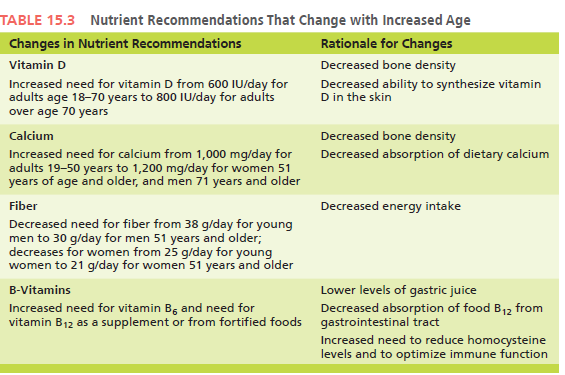
\includegraphics[width=\textwidth]{15_nutrients_that_change_with_increased_age}

\end{figure}

\begin{table}[H]
	\centering
	\caption{Nutrients Recommendations That Change with Increased Age}
	\label{tab:nutrients-that-change-with-increased-age}
	\rowcolors{2}{rowmedgreen}{rowlightgreen}
	\begin{adjustbox}{max width=0.975\paperwidth,center}
		\begin{tabular}{*{2}{p{0.5\paperwidth} }}
			\rowcolor{rowdarkgreen}%
			\textbf{Changes in Nutrient Recommendations} & \textbf{Rationale for Changes}\\
			Vitamin D

			Increased need for vitamin D from 600 IU/day for adults age 18--70 years to 800 IU/day for adults over age 70 years & Decreased bone density

			Decreased ability to synthesize vitamin D In the skin\\
			Calcium

			Increased need for calcium from 1,000 mg/day for adults 19--50 years to 1,200 mg/day for women 51 years of age and older, and men 71 years and older & Decreased bone density


			\rowcolor{rowdarkgreen} & \\
		\end{tabular}
	\end{adjustbox}
\end{table}

\begin{figure}[H]
	\centering
	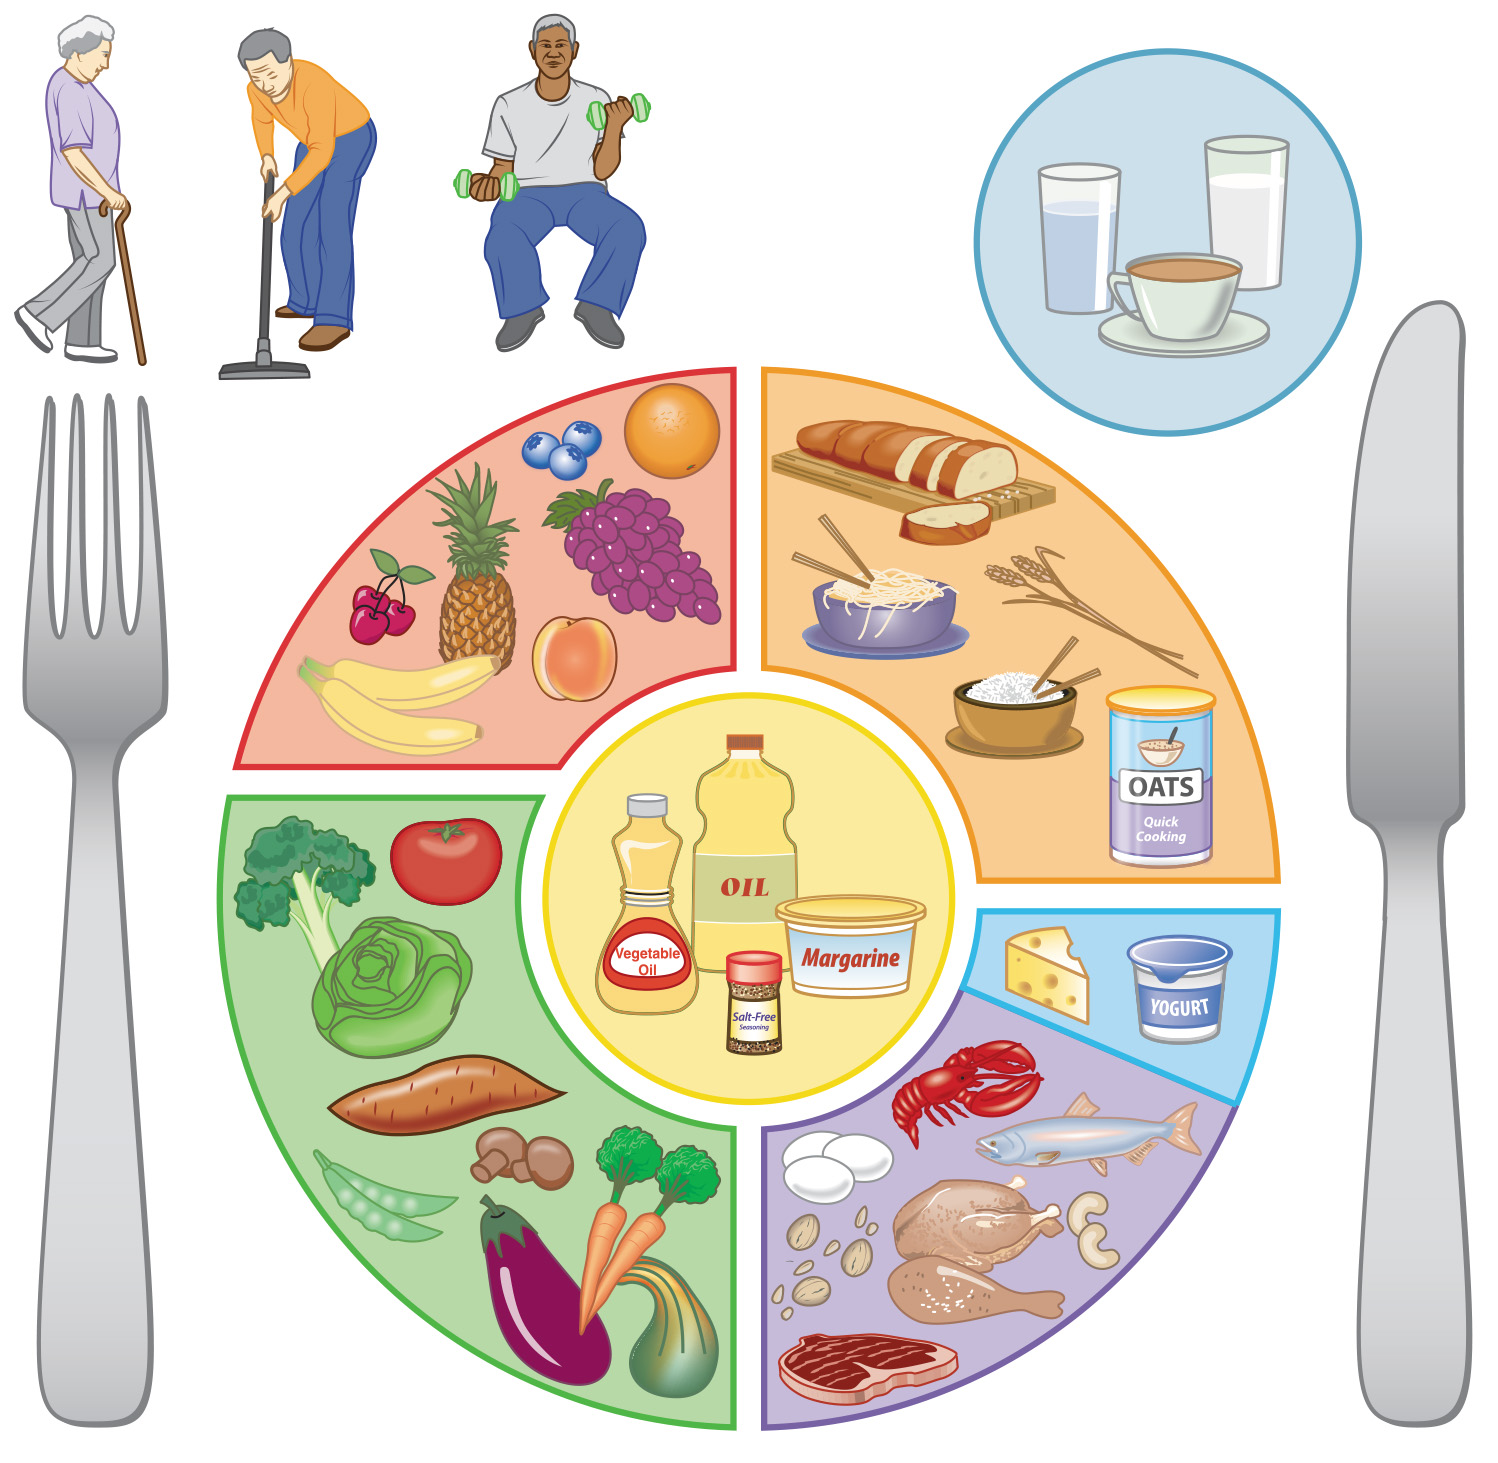
\includegraphics[width=\textwidth]{15_myplate_for_older_adults}
	\caption{MyPlate for Older Adults}
	\label{fig:myplate-for-older-adults}
\end{figure}

\begin{itemize}
	\item Fluid
	\begin{itemize}
		\item AI for fluid is the same as for younger adults
		\begin{itemize}
			\item Men: 3.7 liters/day
			\item Women: 2.7 liters/day
		\end{itemize}
		\item Older adults are especially susceptible to dehydration because changes in kidney function in older adults can impair their thirst mechanism
		\item Important to seek medical attention for incontinence and to drink plenty of fluids
	\end{itemize}
	\item Nutrition-related concerns
	\begin{itemize}
		\item Many chronic diseases are more prevalent in overweight or obese adults
		\item Underweight may result from illness, disability, loss of sense of taste or smell, depression, and social isolation
		\item Dental health issues may cause older adults to avoid meats, firm fruits, and vegetables
	\end{itemize}
\end{itemize}

\begin{figure}[H]
	\centering
	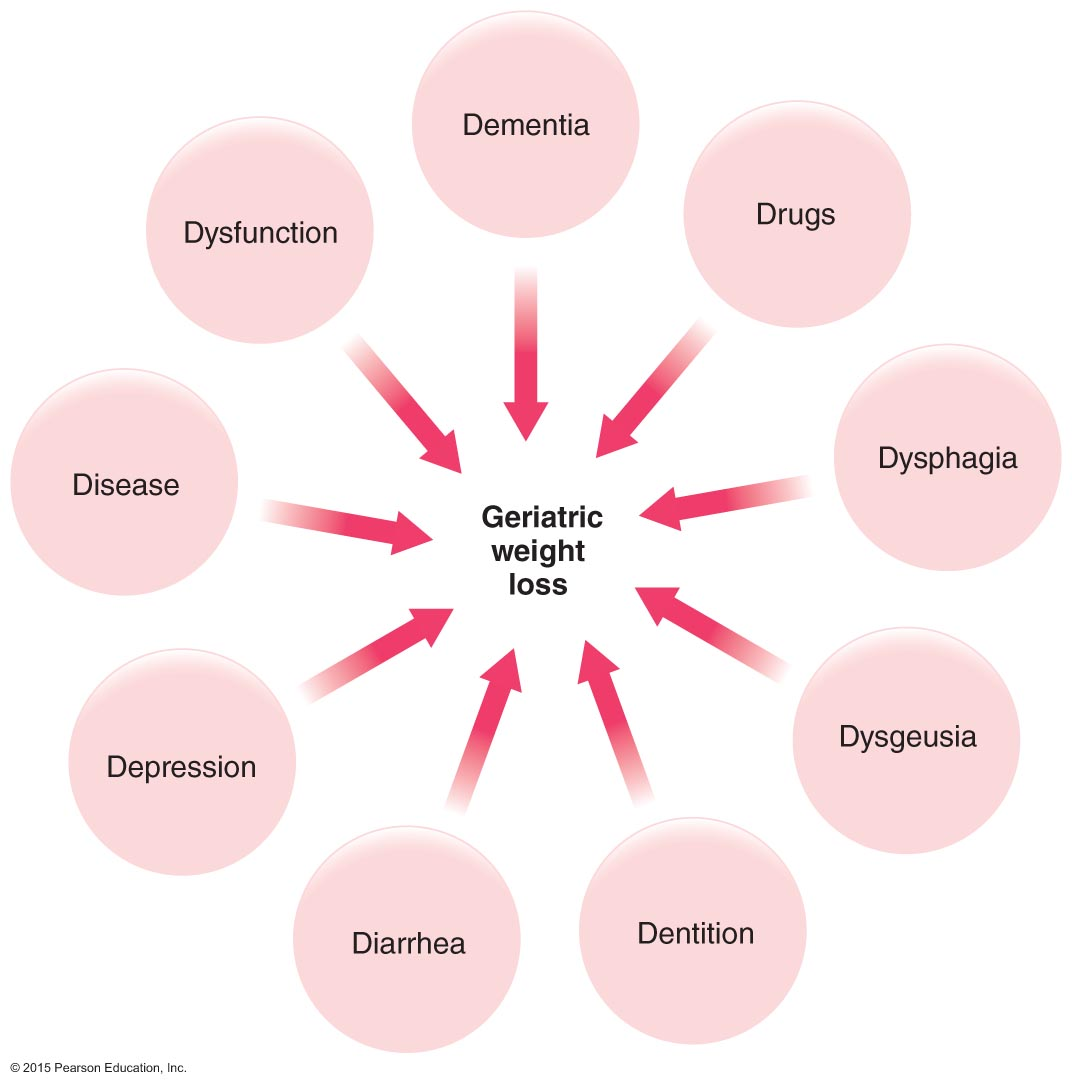
\includegraphics[width=\textwidth]{15_nine_ds_of_geriatric_weight_loss}
	\caption{Nine Ds of Geriatric Weight Loss}
	\label{fig:nine-ds-of-geriatric-weight-loss}
\end{figure}

\begin{itemize}
	\item Nutrition-related concerns
	\begin{itemize}
		\item Age-related eye diseases can cause vision impairment and blindness
		\begin{itemize}
			\item Macular degeneration and cataracts
		\end{itemize}
		\item Some prescription medications can alter nutrient absorption or decrease appetite
		\item Financial and mobility problems
	\end{itemize}
\end{itemize}

\begin{figure}[H]
	\centering
	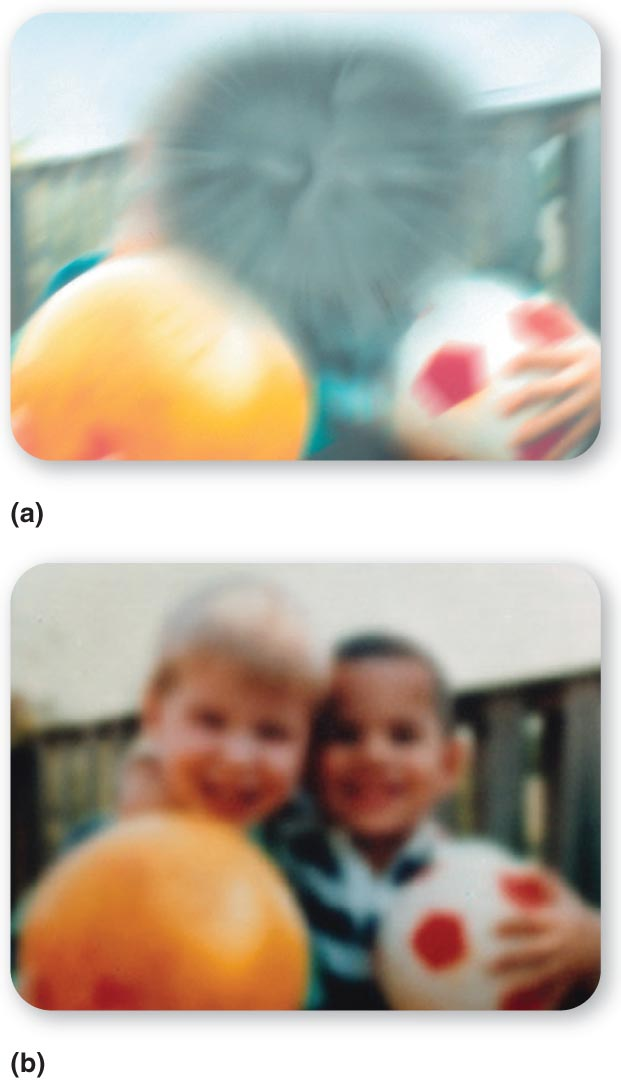
\includegraphics[height=0.75\paperheight]{15_macular_degeneration_and_cataracts}
	\caption{Macular Degeneration and Cataracts}
	\label{fig:macular-degeneration-and-cataracts}
\end{figure}

\begin{figure}[H]
	\centering
	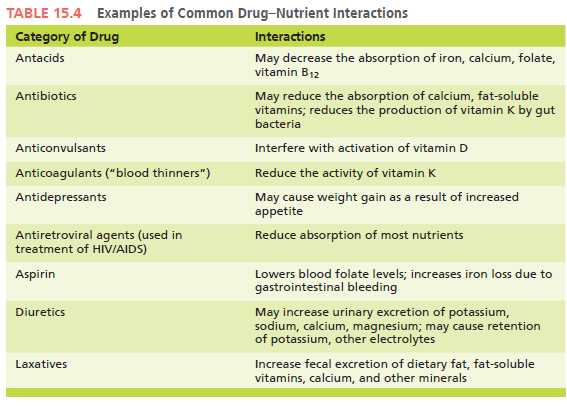
\includegraphics[width=\textwidth]{15_common_drug_nutrient_interactions}
	\caption{Common Drug–Nutrient Interactions}
	\label{tab:common-drug-nutrient-interactions}
\end{figure}

\indepth{The Fountain of Youth}
\begin{itemize}
	\item Growing numbers of people are experimenting with new methods to achieve greater longevity
	\begin{itemize}
		\item Calorie restriction
		\item Intermittent fasting
		\item Supplements
	\end{itemize}
\end{itemize}

\subsection{Calorie restriction (CR)}\label{subsec:calorie-restriction-(cr)}
\begin{itemize}
	\item Researchers have not identified a precise number of Calories to qualify as “restricted”
	\item Typically involves eating fewer Calories than your body needs to maintain normal weight
	\item Should allow for differences in gender, height, age, body composition, activity level, and so forth
	\item Many people practicing CR strive to consume 20–30\% fewer Calories than usual
\end{itemize}

\subsection{Metabolic effects of Calorie restriction}\label{subsec:metabolic-effects-of-calorie-restriction}
\begin{itemize}
	\item Decreased fat mass and lean body mass
	\item Decreased blood glucose levels
	\item Decreased LDL and total cholesterol and increased HDL cholesterol
	\item Decreased core body temperature and blood pressure
	\item Decreased energy expenditure
	\item Decreased oxidative stress
	\item Lower levels of DNA damage
	\item Lower levels of chronic inflammation
	\item Protective changes in some hormone levels
\end{itemize}

\subsection{Challenges of Calorie restriction}\label{subsec:challenges-of-calorie-restriction}
\begin{itemize}
	\item Data are still preliminary
	\item May be ethical concerns for some people’s participation (potential malnutrition)
	\item Much of the data are self-reported from CR groups
	\item May be necessary for CR to last many years to see longevity benefits
	\item Reported side effects include constant hunger, feeling cold, lower sex drive
	\item Long-term effects are not known
\end{itemize}

\subsection{Alternatives to Calorie restriction}\label{subsec:alternatives-to-calorie-restriction}
\begin{itemize}
	\item Intermittent fasting (IF):
	\begin{itemize}
		\item Alters the pattern of food consumption
		\item Has shown positive effects in animals
		\item May be tolerable for more people
	\end{itemize}
	\item Limiting total protein intake
	\item Exercise-induced leanness
\end{itemize}

\subsection{Supplements}\label{subsec:supplements}
\begin{itemize}
	\item The ``anti-aging'' market is rife with supplements making longevity claims
	\item No research trials to date have shown a clear connection between increased nutrient intake from supplements and lower rates of death
	\item Greatly increased nutrient intake levels may pose dangers to some people
	\item Many non-nutrient supplements (such as gingko, DHEA) can have potentially serious side effects
\end{itemize}

\begin{itemize}
	\item \textit{Proven} things you can do to increase your chances of living a long and healthful life:
	\begin{itemize}
		\item Get regular physical activity
		\item Eat nutritious, balanced meals
		\item Take only supplements recommended by a qualified healthcare provider, in only the amounts recommended
		\item Maintain a healthful body weight
		\item Don’t smoke or use tobacco products
		\item Consume alcohol in moderation
	\end{itemize}
\end{itemize}
%</Chapter15>

\end{document}
